% Created 2024-07-21 Sun 23:54
% Intended LaTeX compiler: xelatex
\documentclass[a4paper,11pt,twoside]{article}
\usepackage{graphicx}
\usepackage{longtable}
\usepackage{wrapfig}
\usepackage{rotating}
\usepackage[normalem]{ulem}
\usepackage{amsmath}
\usepackage{amssymb}
\usepackage{capt-of}
\usepackage{hyperref}
\usepackage{libertine} \usepackage{amsmath}
\usepackage[width=200.00mm, height=240.00mm, left=3cm, right=3cm, top=3 cm, bottom=3cm]{geometry}
\usepackage{graphicx}
\graphicspath{ {./images/} }
\usepackage{multicol}
\author{Ryan P. Lynch}
\date{\today}
\title{Program 2B}
\hypersetup{
 pdfauthor={Ryan P. Lynch},
 pdftitle={Program 2B},
 pdfkeywords={},
 pdfsubject={},
 pdfcreator={Emacs 29.4 (Org mode 9.6.24)}, 
 pdflang={English}}
\usepackage{biblatex}

\begin{document}

\maketitle
\section*{Compile and Executing MFQ}
\label{sec:orgbd330cd}
The below screen shots are from compiling \emph{Scheduler\textsubscript{mfq.java}}
\begin{verbatim}
mv Scheduler_mfq.java Scheduler.java
javac -deprecation Scheduler.java
\end{verbatim}
Sending the starting exec to the scheduler.
\begin{center}
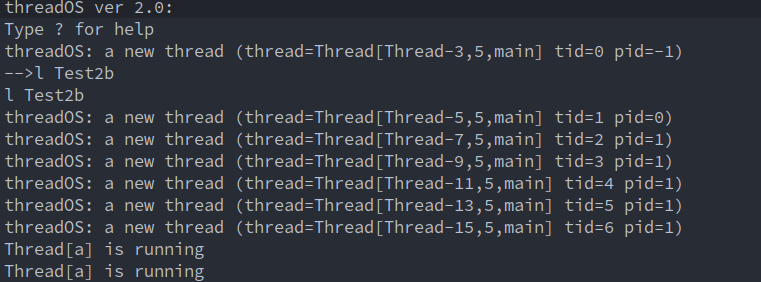
\includegraphics[width=.9\linewidth]{./mfq0.png}
\end{center}
The first result from finished thread.
\begin{center}
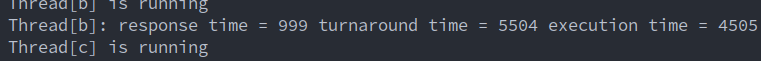
\includegraphics[width=.9\linewidth]{./mfq1.png}
\end{center}
The second result from finished thread.
\begin{center}
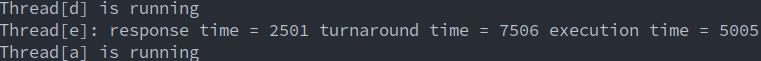
\includegraphics[width=.9\linewidth]{./mfq2.png}
\end{center}
The third result from finished thread.
\begin{center}
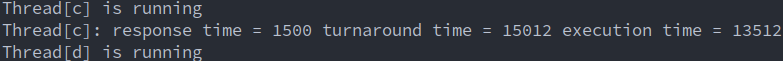
\includegraphics[width=.9\linewidth]{./mfq3.png}
\end{center}
The fourth result from finished thread.
\begin{center}
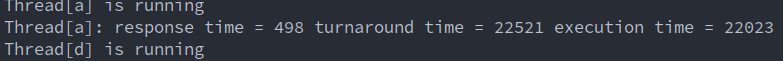
\includegraphics[width=.9\linewidth]{./mfq4.png}
\end{center}
The fifth and final result from finished thread.
\begin{center}
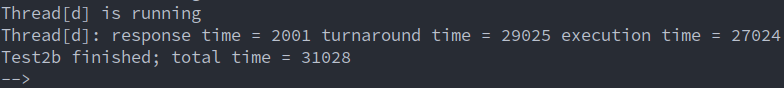
\includegraphics[width=.9\linewidth]{./mfq5.png}
\end{center}
\subsection*{Runtime Table}
\label{sec:orga248a39}
\begin{center}
\begin{tabular}{lrrrl}
 & Response & TAT & Exec Join & Total\\[0pt]
\hline
b & 999 & 5504 & 4505 & \\[0pt]
e & 2501 & 7506 & 5005 & \\[0pt]
c & 1500 & 15012 & 13512 & \\[0pt]
a & 498 & 22521 & 22023 & \\[0pt]
d & 2001 & 29025 & 27024 & \\[0pt]
\hline
avg. & 1499.8 & 15913.6 & 14413.8 & 31028\\[0pt]
\end{tabular}
\end{center}
\section*{Compile and Executing RR}
\label{sec:org01dc5ba}
The below screen shots are from compiling \emph{Scheduler\textsubscript{rr.java}}
\begin{verbatim}
mv Scheduler_rr.java Scheduler.java
javac -deprecation Scheduler.java
\end{verbatim}
Sending the starting exec to the scheduler.
\begin{center}
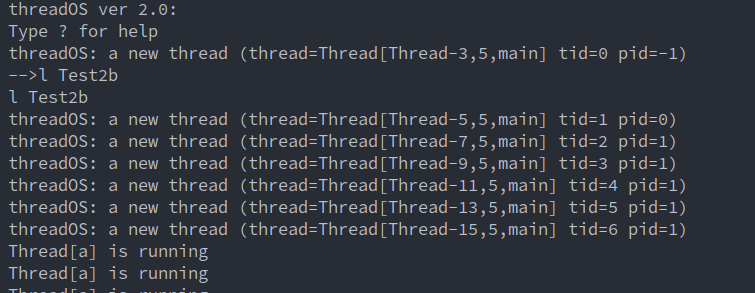
\includegraphics[width=.9\linewidth]{./rr0.png}
\end{center}
The first result from finished thread.
\begin{center}
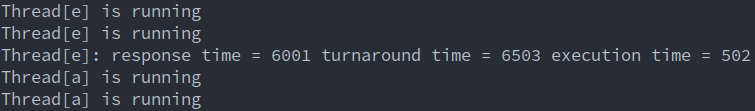
\includegraphics[width=.9\linewidth]{./rr1.png}
\end{center}
The second result from finished thread.
\begin{center}
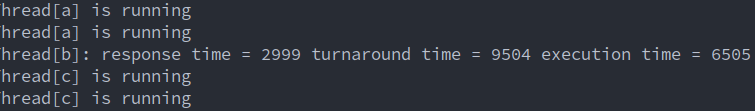
\includegraphics[width=.9\linewidth]{./rr2.png}
\end{center}
The third result from finished thread.
\begin{center}
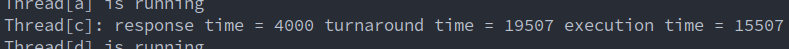
\includegraphics[width=.9\linewidth]{./rr3.png}
\end{center}
The fourth result from finished thread.
\begin{center}
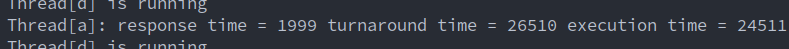
\includegraphics[width=.9\linewidth]{./rr4.png}
\end{center}
The fifth and final result from finished thread.
\begin{center}
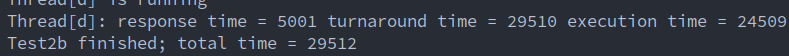
\includegraphics[width=.9\linewidth]{./rr5.png}
\end{center}
\subsection*{Runtime Table}
\label{sec:orgd169b5b}
\begin{center}
\begin{tabular}{lrrrl}
 & Response & TAT & Exec Join & Total\\[0pt]
\hline
e & 6001 & 6503 & 502 & \\[0pt]
b & 2999 & 9504 & 6505 & \\[0pt]
c & 4000 & 19507 & 15507 & \\[0pt]
a & 1999 & 26510 & 24511 & \\[0pt]
d & 5001 & 29510 & 24509 & \\[0pt]
\hline
avg. & 4000 & 18306.8 & 14306.8 & 29512\\[0pt]
\end{tabular}
\end{center}
\end{document}
